\documentclass[11pt,a4paper]{article}

\usepackage{amsmath} %for mathemathic formulas
\usepackage{amssymb}
\usepackage[ngerman]{babel} %for the german language by the spellling reform (without the package the date would look like April 20, 2020)
\usepackage{enumitem} %for enumeration surrounding 
\usepackage{graphicx} %for pictures
\usepackage{siunitx}
\usepackage{float}

\title{Blatt 4}
\date{\today}
\author{Hannah Rotgeri \and Feline Heinzelmann}

\begin{document}
    \maketitle

    \section*{Aufgabe 1}
	\begin{itemize}
		\item[a)]
			Für einen planaren Undulator ergibt sich durch eine alternierende Anordnung von Magneten ein transversales und longitudinales cosinus- bzw. sinusförmiges B-Feld. 
			Dazu senkrecht bildet das E-Feld in Sinus- bzw. Cosinusform aus (elektromagnetische Induktion).
		\item[b)]
			Das elektrische Feld besteht als Überlagerung vieler sinusförmiger Wellen des E-Feldes aus verschiedenen Wellenlängen bzw. Frequenzen, wobei es eine Grundschwingung gibt.
			Die Fouriertransformierte des E-Feldes trennt diese Überlagerungen auf, wodurch im Spektrum, Betragsquadrat des E-Feldes bzw. des fouriertransformierten E-Feldes, 
			die verschiedenen Frequenzsanteile dargestellt werden. Das sich ergebende Spektrum bezeichnet sich als Linienspektrum. 
			Die Linienform wird mit zunehmender Breite $N$ schmaler als Eigenschaft der Fourier-Transformierten.
	\end{itemize}


	
    \section*{Aufgabe 2}

	\begin{itemize}
		\item[a)]
		\begin{align*}
			\lambda &= \frac{\lambda_{u}}{2 \gamma^{2}} \cdot (1 + \frac{K^2}{2} + \gamma^2 \theta^2) \text{ mit } \theta = 0 \\
						&= \frac{\lambda_{u}}{2 \gamma^{2}} \cdot (1 + \frac{K^2}{2} ) \\ 
						&= \SI{8.7e-9}{\meter} \text{ für } K = 1, \\
						&= \SI{0.12e-9}{\meter} \text{ für } K = 1.5, \\
						&= \SI{0.17e-9}{\meter} \text{ für } K = 2, \\
						\\
			E_{\mathrm{Photon}} &= h \cdot \frac{c}{\lambda} \\
									&= \SI{142}{\electronvolt} \text{ für } K = 1, \\
									&= \SI{101}{\electronvolt} \text{ für } K = 1.5, \\
									&= \SI{71}{\electronvolt} \text{ für } K = 2			
		\end{align*}        	
        \item[b)]
			
	\end{itemize}


    \section*{Aufgabe 3}
		\begin{itemize}
			\item[a)] Betragsquadrat des elektrischen Felds (wieder in willkürlichen Einheiten) als Funktion der Photonenenergie 
			im Bereich von $\SI{1}{\electronvolt} \, \text{bis} \, \SI{450}{\electronvolt}$:
			\begin{figure}[H]
				\centering
				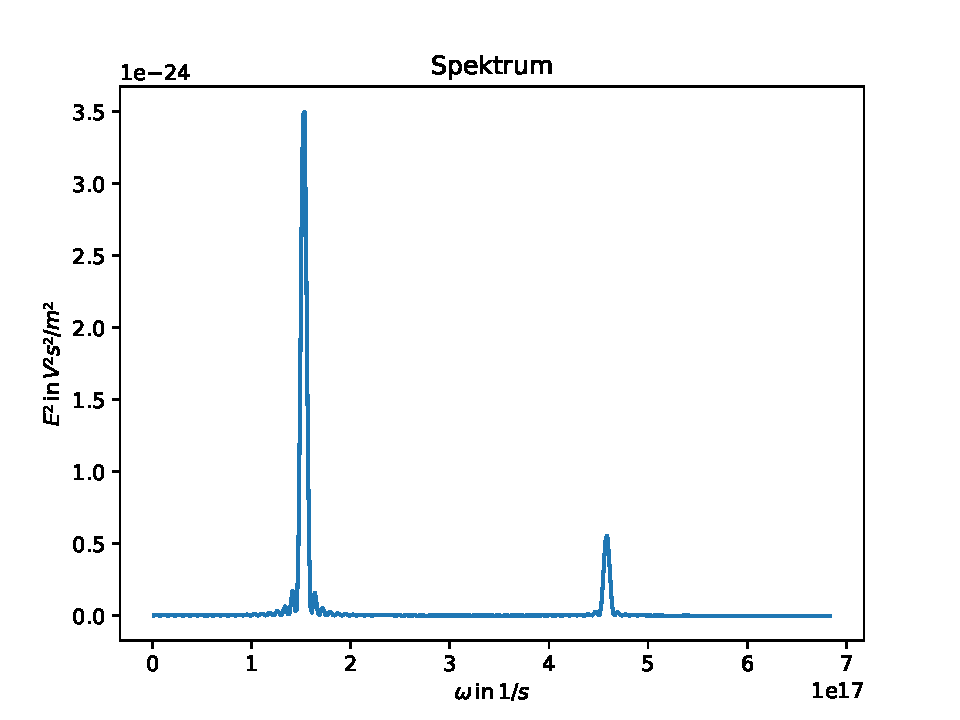
\includegraphics[width=0.5\textwidth]{build/spektrum_K1.5_Perioden20_neu.pdf}
			\end{figure}

			\item[b)] Spektrum auch für 10 und 40 Undulatorperioden:

			\begin{figure}[H]
				\centering
				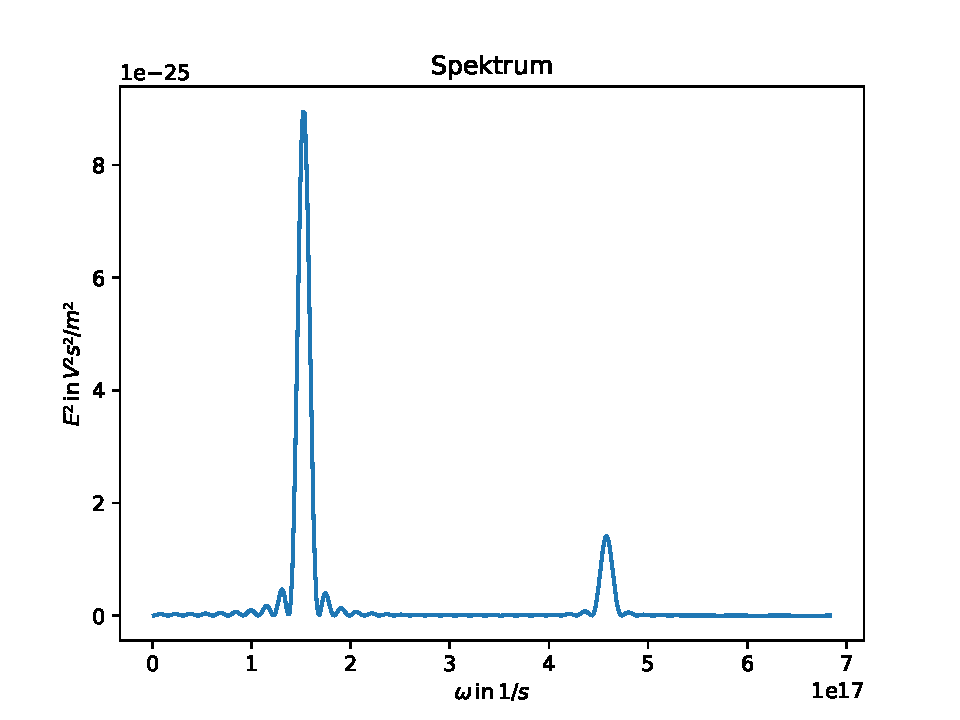
\includegraphics[width=0.5\textwidth]{build/spektrum_K1.5_Perioden10_neu.pdf}
				\caption{$T = 10$}
			\end{figure}

			\begin{figure}[H]
				\centering
				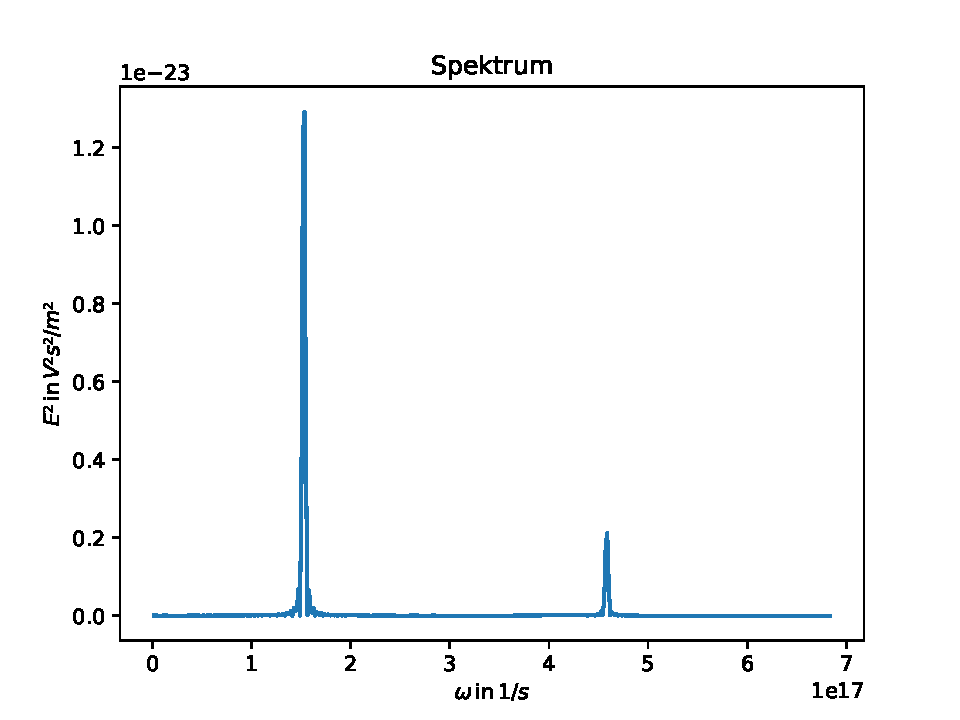
\includegraphics[width=0.5\textwidth]{build/spektrum_K1.5_Perioden40_neu.pdf}
				\caption{$T = 40$}
			\end{figure}

			Mit zunehmender Periodendauer kann man eine Stauchung des Spektrums beobachten, d. h. ein schmalbandigeres Spektrum 
			bezüglich der Kreisfrequenz.

			\item[c)] Spektrum für $K = 1$ und $K = 2$:
			\begin{figure}[H]
				\centering
				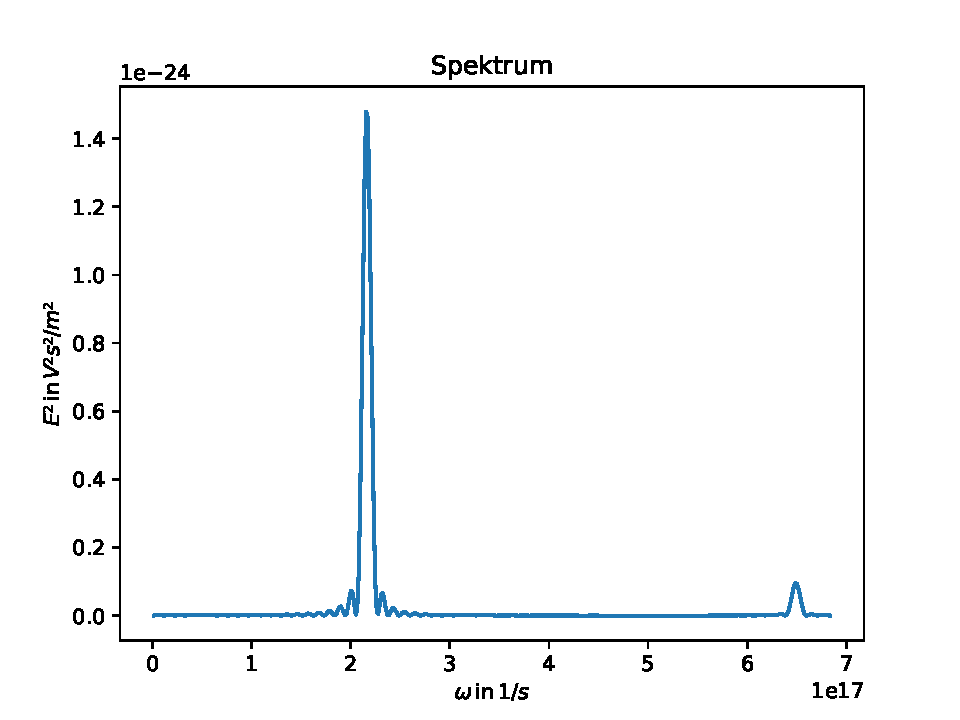
\includegraphics[width=0.5\textwidth]{build/spektrum_K1.0_Perioden20_neu.pdf}
				\caption{$K=1$}
			\end{figure}

			\begin{figure}[H]
				\centering
				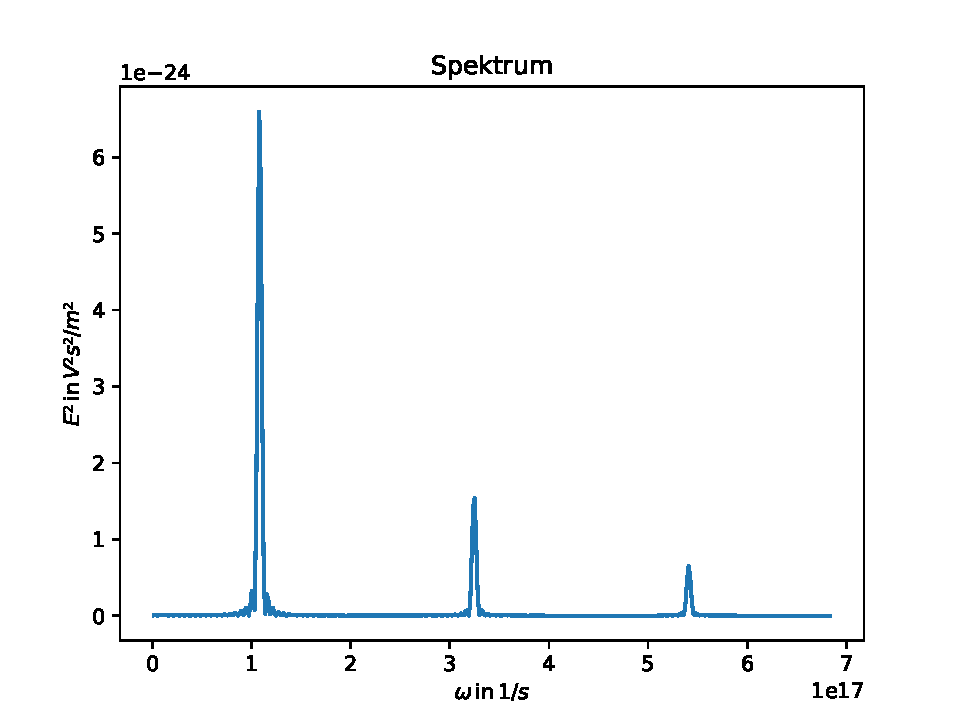
\includegraphics[width=0.5\textwidth]{build/spektrum_K2.0_Perioden20_neu.pdf}
				\caption{$K=2$}
			\end{figure}

			Mit zunehmendem Undulatorparamter K ergeben sich mehr Peaks im Spektrum. Der erste und höchste Peak, auch erste Harmonische genannt, ergibt sich durch konstruktive Interferenz 
			wegen kohärenter Überlagerung eines Photons mit einem, das an der nächsten Periode emittiert wird. Die anderen Peaks sind Oberschwingungen, d. h. höhere Harmonische, die ein
			Beobachter auf der Undulatorachse sieht. Mit zunehmendem $K$ entstehen ungeradzahlige Harmonische.
		

			\item[d)] Spektrum unter Annahme einer konstanten longitudinalen Elektronengeschwindigkeit $\beta^{*}$:

			\begin{figure}[H]
				\centering
				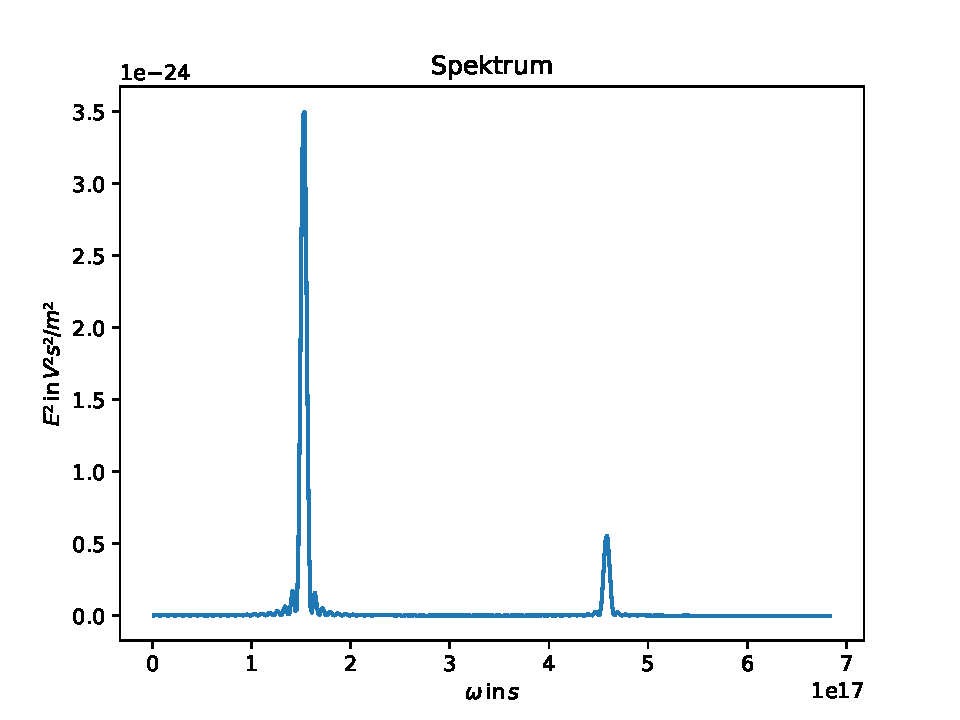
\includegraphics[width=0.5\textwidth]{build/spektrum_K1.5_Perioden20_d.pdf}
			\end{figure}

			Das Spektrum bleibt bezüglich einer Veränderung der longitudinalen Geschwindigkeitskomponente unverändert.

		\end{itemize}







\end{document}


